\section{What is machine learning?} \label{ch:what_is_ml}

\subsection{Machine learning in general}

Usually the task of programming is to apply rules to certain problems in order to obtain solutions.
With the help of machine learning we want to create a model that uses solutions for certain problems to find out the corresponding rules.
The relationship is shown in figure~\ref{fig:cp_vs_ml}.

\begin{figure}
    \centering
    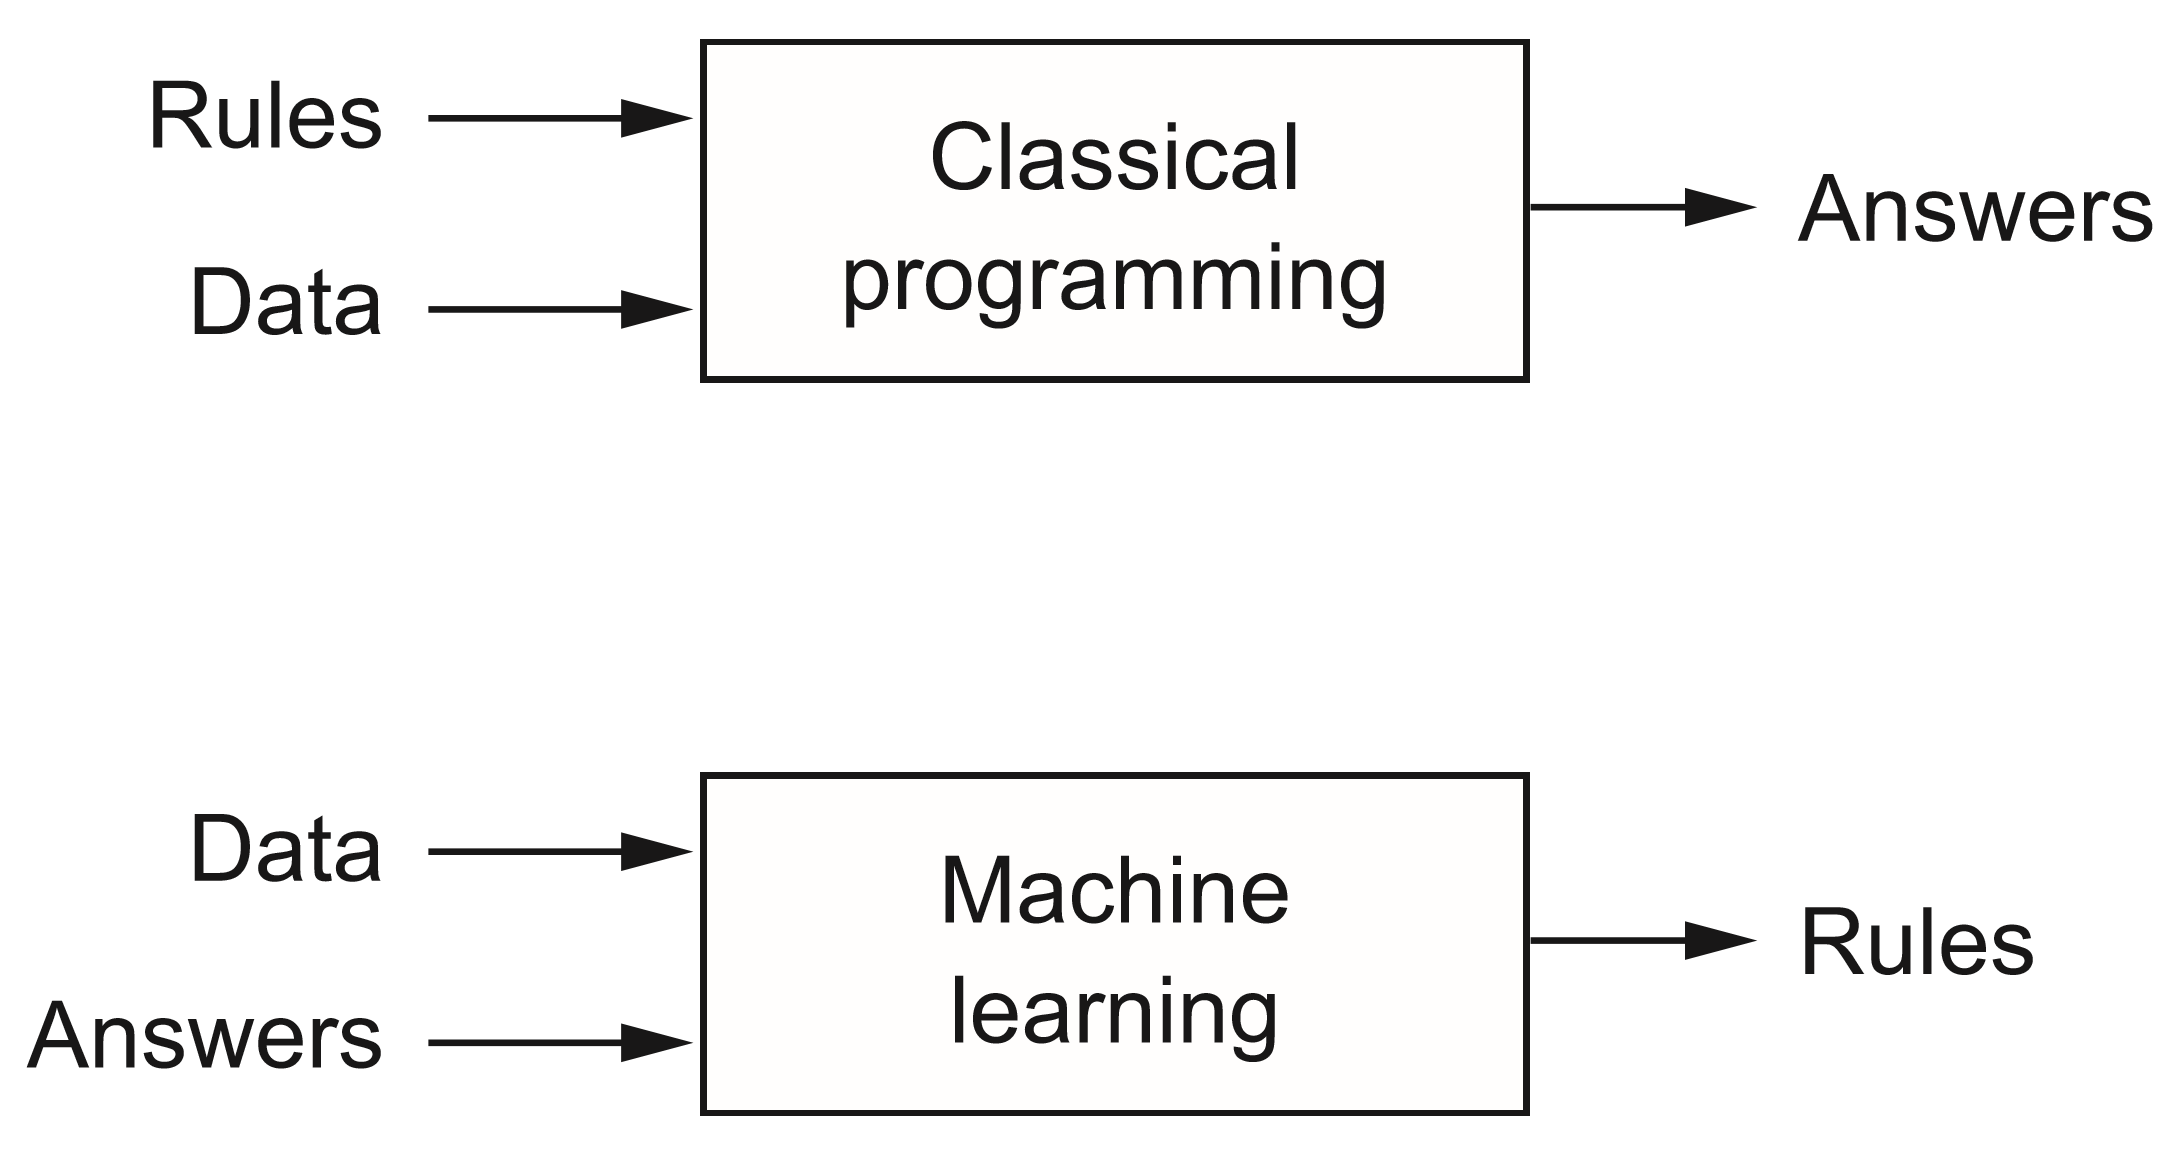
\includegraphics[width=0.5\textwidth]{images/classical_prog_vs_ml.png}
    \caption[ML, a new programming paradigm]{Machine learning, a new programming paradigm \cite[p.5]{Chollet2017}}
    \label{fig:cp_vs_ml}
\end{figure}

The promise of machine learning is that the rules learned can be much more complex than it is possible to program by hand.
A good example is image recognition (which will be the focus of this project), where the content of images is to be classified.
The relations between the pixels have to be found out, which leads to a rather complex model.
This cannot be programmed in the traditional way even for the simplest tasks.

The universal approximation theorem \cite{Cybenko1989, Hornik1989} states that for any input $x$ there is a function $h$ which approximates the mapping $y$, while the mapping is only the input to the correct output (often labeled by a human).
This relationship is described in equation~\eqref{eq:universal_approx}.

% TODO define sets X and Y of \theta and x
\begin{equation}
    \forall \epsilon > 0 :
    \exists h(\theta, x) : \forall x \in I : | h(\theta, x) - y(x) | < \epsilon
    \label{eq:universal_approx}
\end{equation}
% TODO the text here can be changed with a class of functions (see UAT paper)

The mathematical description of $h$ is called a model (e.g. $h(x) = \sum_{i=1}^n{\lambda (\theta^T * x)}$).
$\lambda \in \mathbb{R}$ is a constant and $\theta$ is a tensor that defines the parameters of $h$, which are made up of so-called weights and biases, which will be explained later.

The universal approximation theorem makes no statements about the form of $\theta$; therefore $h$ is called a hypothesis because it states that for a certain composition of $\theta$ this equation is true.
This term is summarized in the equation~\eqref{eq:hypothesis}.

\begin{equation}
    \forall \epsilon > 0 : \exists \theta \in X : \forall x \in I : |
    h_\theta(x) - y(x) | < \epsilon
    \label{eq:hypothesis}
\end{equation}

A loss function is used for model valuation; it compares the result of the hypothesis with the data provided.
Probably the most prominent loss function is the \name{mean square error}.
It takes the sum of the deviation of $n$ examples squared and divides it by $2*n$.

\begin{equation}
    L_{mse}(\theta, x) = \frac{1}{2 n} \sum_{i=1}^n (h_\theta(x) - y(x))^2
    \label{eq:mse}
\end{equation} 

The task of machine learning is to determine a $\theta$ for a model that confirms the equations~\ref{eq:universal_approx} and \ref{eq:hypothesis}, which is done by iterative updating of $\theta$. 
Before training, $\theta$ is randomly initiated and then iteratively adjusted to make $\epsilon$ converge toward zero. This minimizes the value of $L$.

In order for the value of the loss function to gradually decrease, $\theta$ is adjusted using an optimization function.
This is usually done with a gradient descent algorithm or a variant of it.
The gradient descent is performed by calculating the gradient of the loss function and subtracting it from the corresponding parameters shown in equation~\eqref{eq:gradient_descent}.

\begin{equation}
    \theta_{i+1} := \theta_i - \eta \nabla_\theta L(\theta, x)
    \label{eq:gradient_descent}
\end{equation}

Where $\eta$ is a constant called the learning rate, which helps the loss function converge to 0 using the gradient descent algorithm.
It is one of many hyperparameters that are not automatically adjusted during training, but are determined beforehand.
Optimal adjustment of hyperparameters is an important task that is difficult to automate and is therefore the focus of much research\footnote{There are algorithms for adjusting the learning rate, namely \name{AdaGrad} \cite{Duchi2010} and derived algorithms and is the main topic of the chapter \ref{ch:hyper_parameter_tuning}}.
If the equation \eqref{eq:hypothesis} applies to the model in question, it is then sufficiently suitable for the given input.

These concepts are presented now using a simple example.

\subsection{Simple linear example} \label{ch:simple_linear_example}

As an illustrative example, a model is created that translates Fahrenheit into Celsius\footnote{Please note that using a learning algorithm here is very inefficient and is in contrast to Maslow's hammer (\aka{https://en.wikipedia.org/wiki/Law_of_the_instrument}).}.
The original equation is given by the linear function $y = mx + b$ as $F = C * 1.8 + 32$, with $F$ as degrees Fahrenheit and $C$ as degrees Celsius.

A model to learn this relationship is defined in the listing~\ref{lst:c_to_f} \footnote{Also available at \aka{https://klawr.github.io/deepmech/reports/srp/demos/c_to_f.js}} .

% TODO add JavaScript as language
\lstinputlisting[label={lst:c_to_f}, caption={Celsius to Fahrenheit}]{code/c_to_f.js}

The described model is implemented by \code{w} and the hypothesis function by \code{h}.
Since it is known that the relationship is linear, the model represents a one-dimensional polynomial, with the first index being dimensionless (and, as mentioned above, emulating the bias) and the second being used as input x.
We will add a dimension later to demonstrate the behavior with polynomials that do not directly represent the target function.

\code{y} provides the correct, predefined solution.
Please note that \code{y} is only used during training and is omitted if the model parameters are correctly set after training.

In this example the loss function is described by the \textit{mean square error } \footnote{ Abbreviated as \textit{mse}, which is shown in equation \eqref{eq:mse}}.

To minimize the loss function gradient descent described in equation~\eqref{eq:gradient_descent} is used.

In listing~\ref{lst:c_to_f} equation~\eqref{eq:gradient_descent} is implemented as \code{sgd} with $\theta_0 = \code{b}$ and $\theta_1= \code{m}$ as shown in equation~\eqref{eq:sgd_mse_here}.

\code{sgd} is short for \textit{stochastic gradient descent}\footnote{A distinction is made between batch, mini-batch and stochastic gradient descent; using a complete data set, a defined subset or individual data on the individual iterations of the training process}.
It represents the optimization function that updates the parameters of the model by calculating the gradient of loss for each parameter and then updating it.

\begin{equation}
    \begin{split}
        \theta_{0} & := \theta_{0} - \frac{\partial L}{\partial \theta_{0}} =
        \theta_{0} - (h(x) - y(x))  \\
        \theta_{1} & := \theta_{1} - \frac{\partial L}{\partial \theta_{1}} =
        \theta_{0} - (h(x) - y(x)) * x
    \end{split}
    \label{eq:sgd_mse_here}
\end{equation}

\begin{lstlisting}[caption={Output of C to F converter.}]
loss:  343041.666256673
loss:  16242.7707476548
loss:  88.27595280422442
loss:  10.74432403839251
loss:  1.1607137779951606
loss:  0.252186283500194
loss:  0.00040450626910586374
loss:  0.00004247033303206121
loss:  7.158429555712516e-7
loss:  1.6948019668728757e-10
weights:  [ 31.99999973758735, 1.8000003977458756 ]
\end{lstlisting} 

The expected behavior for the loss function is to decrease with each iteration.
This is the case in this example, showing that the deviation of the hypothesis from the actual result decreases.
After 200 iterations, the parameters \code{m} and \code{b} of the \code{model} are displayed and show that they are actually close to the expected result.
By increasing the number of iterations, the result can be increased up to the point where they are rounded by the JavaScript compiler to represent exact results (using Node.js\footnote{As far as can be assumed when calculating exact results using floating point numbers.}).

\begin{SCfigure}
    \centering
    \caption[Simplest model]{This example can be visualized as shown here. The bias can be interpreted as additional input, which always has the value 1. The input is multiplied by the parameters marked with the corresponding arrows, which in turn are summed up (resulting in $y = mx + b$).}
    
\includegraphics[width=0.45\textwidth]{images/1_simplest_nn.png}
\end{SCfigure} 

Provided that this hypothesis is initially well suited to the task, it is important to note that by modifying the hypothesis to represent a polynomial of higher degree (e.g. $y = nx^2 + mx + b$) the additional parameters converge towards 0, which effectively gives the same result as before \footnote{But to achieve similar results, the iteration number must be increased by at least a factor of 20}.

The experiment can be followed at \aka{https://klawr.github.io/deepmech/reports/srp/demos/c_to_f_adv.js}.
